\documentclass{article}

\usepackage{caption}
\usepackage{csquotes}
\usepackage[margin=0.7in]{geometry}
\usepackage{graphicx}
\usepackage{rotating}
\usepackage{float}
\usepackage[section]{placeins}
\usepackage{sectsty}
\sectionfont{\clearpage}

\usepackage{xcolor}
\usepackage{listings}
\lstset{
	language=Verilog,
	frame=single,
	basicstyle=\small,
	keywordstyle=\color{blue}\small,
	stringstyle=\color{Maroon}\small,
	commentstyle=\color{OliveGreen}\small,
	breaklines=true,
	postbreak=\raisebox{0ex}[0ex][0ex]{\ensuremath{\color{red}\hookrightarrow\space}}
}


\title{FPGABoy Documentation}
\author{Luke Wren}

\begin{document}

\pagenumbering{gobble}
\maketitle
\tableofcontents
\newpage
\pagenumbering{arabic}

\section{What?}

FPGABoy is an open source portable games console, designed from scratch. It is also...
\begin{itemize}
\item An open source PCB layout
\item Designed with KiCAD open source PCB editor
\item An open source CPU, graphics and bus architecture
\item Based on the RISC-V open source instruction set
\item Synthesised and taped out with iCEStorm open source FPGA toolchain
\end{itemize}

\begin{displayquote}
\textit{If you say open source one more time I'm gonna nut instantly} - Oscar Wilde
\end{displayquote}

\subsection{Logic Design}

\begin{figure}[!htb]
\caption{System-level architecture}
\label{diagram:system_arch}
\centering
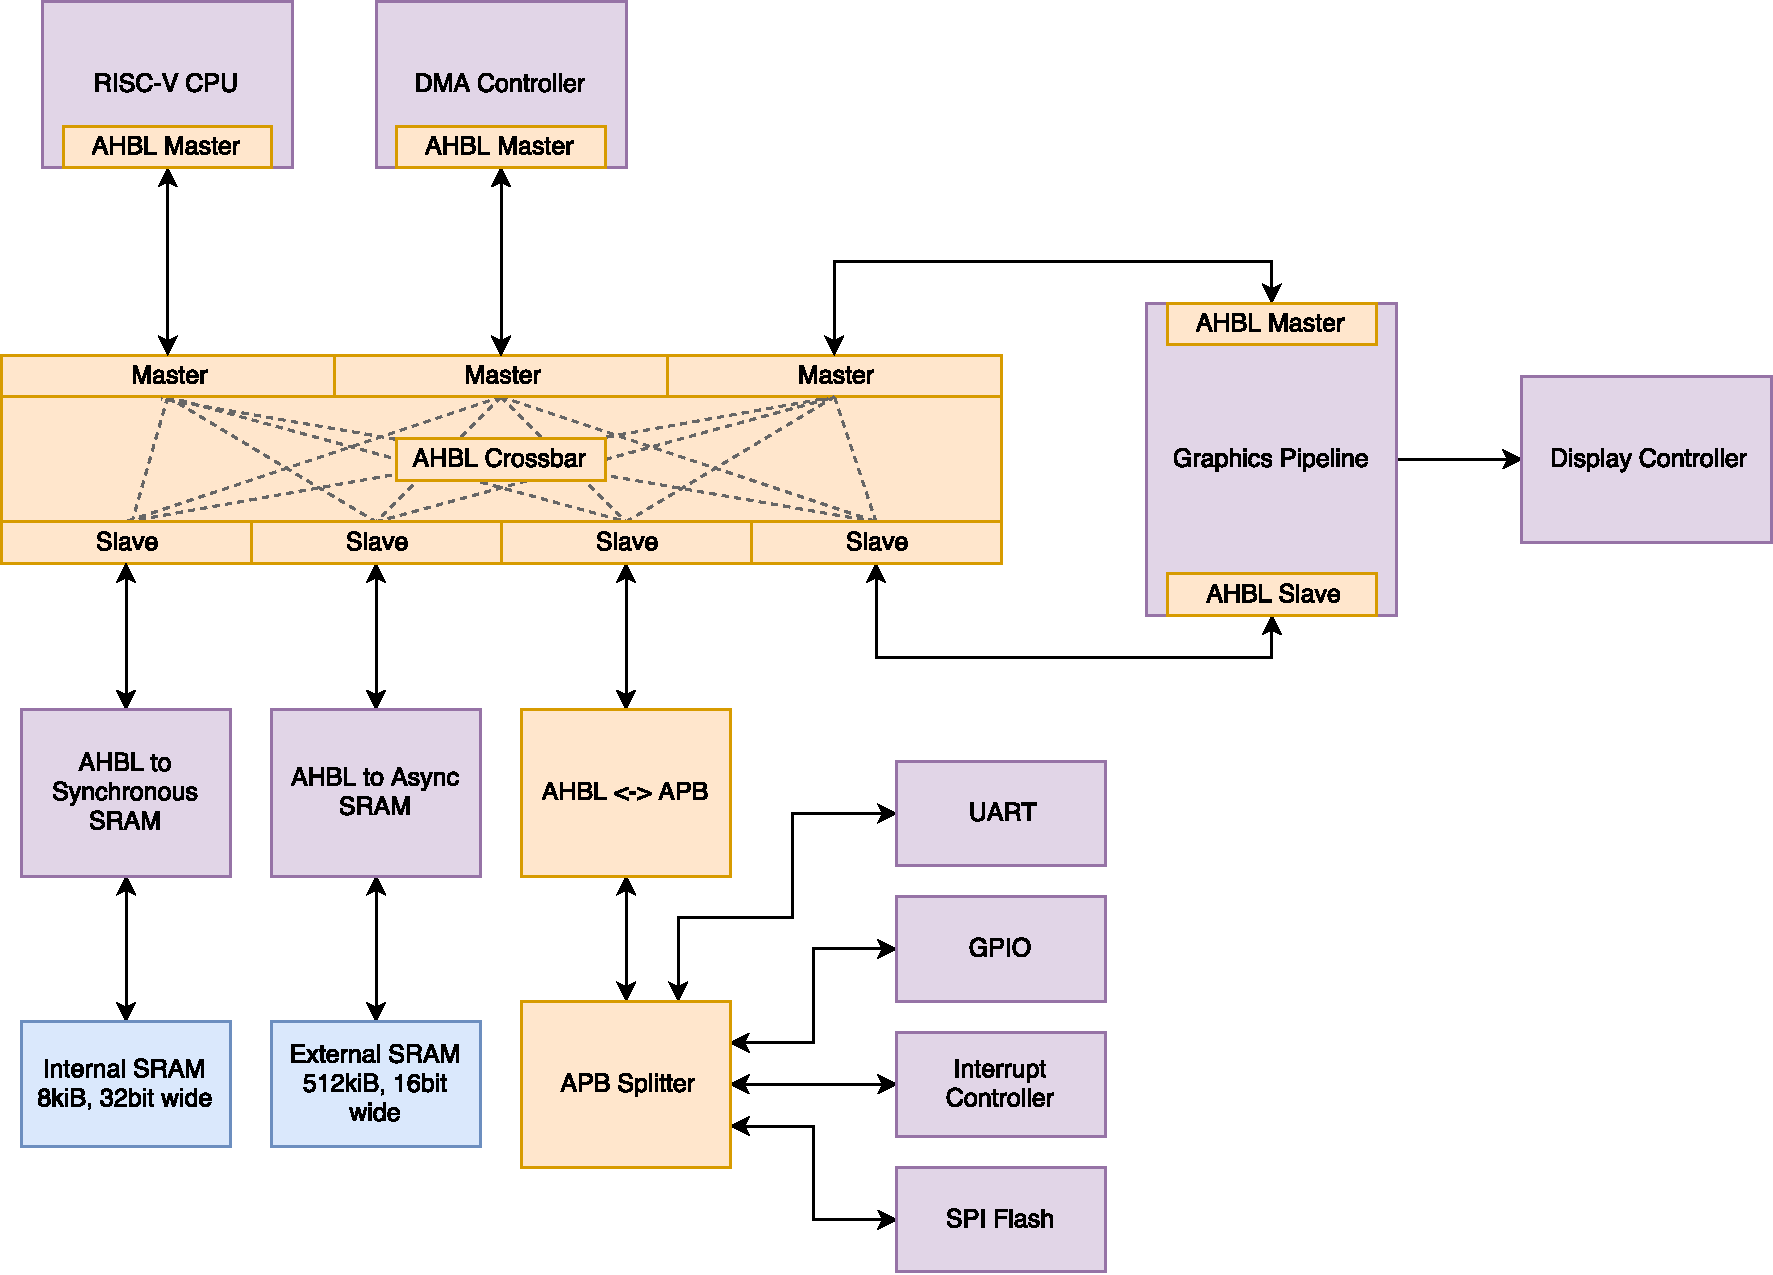
\includegraphics[width=0.7\textwidth]{diagrams/system_arch.pdf}
\end{figure}

The heart of the design is a Lattice iCE40-HX8k FPGA, containing 7680 LUT4s and flipflops. The logic was designed from scratch, using synthesisable Verilog. This includes:
\begin{itemize}
\item RV32IC-compatible 32-bit CPU design
	\begin{itemize}
	\item RISC-V instruction set
	\item 32I: base integer ISA profile
	\item C: compressed instruction extension, for higher code density
	\end{itemize}
\item Graphics pipeline
	\begin{itemize}
	\item Don't expect much, it's about as powerful as a Gameboy Advance
	\item Includes some MODE7-like functionality which allows drawing perspective-mapped textured planes, by providing per-scanline affine texture transformation. Think MarioKart
	\end{itemize}
\item AHB Lite 3.0-compatible multi-master busfabric
\item Other peripherals
	\begin{itemize}
	\item External SRAM controller
	\item Display controller
	\item DMA master
	\item Interrupt controller
	\item GPIO controller (buttons!)
	\item Serial port etc.
	\end{itemize}
\end{itemize}

Some attempt is made in this document to describe the operation of these hardware blocks, but if you are looking for nitty-gritty detail, the best documentation is the files ending with \texttt{.v}.

That a free synthesis tool can cram all this logic into one of the cheapest FPGAs on the market is tremendously impressive. Hopefully we will one day have a situation similar to software compilers, where free tools such as GCC are industry standards.

\subsection{PCB}

The board is a 4-layer stackup:

\begin{enumerate}
\item Signal + GND Fill
\item GND plane
\item Power planes
\item Signal + GND Fill
\end{enumerate}

It is intended to be suitable for low-cost PCB prototyping services such as iTead. Board dimensions are 50mm $\times$ 50mm, which fits into the cheapest size category on iTead. For the most part, it sticks to the following minimum specifications:

\begin{itemize}
\item Track width 0.15mm
\item Copper-copper clearance 0.15mm
\item Soldermask-copper clearance 0.1mm
\item Soldermask width 0.1mm
\item Via drill 0.3mm
\item Annular ring 0.15mm (i.e. via diameter 0.6mm)
\end{itemize}

The only exception is some 0.5mm vias underneath the BGA. Strictly this is out of specification for iTead, but they claim to have a 90 $\mu$m drill registration, so we'll see how it goes.

The iCE40-HX8k FPGA is packaged in a 256-pin 0.8mm BGA, which \textit{can be} reflowed by a hobbyist with a hot air gun or a frying pan (best to choose a HASL finish so that contacts are pretinned). The 132-pin 0.5mm BGA has sufficient IO for our needs, but iTead does not manufacture at the tolerance required for such a fine pitch.


\subsection{Licensing}

The Verilog source to this project has no dependencies, and is distributed under the DWTFPL version 3. This is a very... permissive open-source licence, and its text should be included in full at the top of the source files.


\section{CPU Architecture}

ReVive is a 32-bit processor based on the RISC-V instruction set architecture. It yearns for the glory days of games programming, when NULL pointers were just pointers to the start of ROM, and programmers were real programmers who wrote their \textit{own} polygon rasterisers, dammit. Targeting a small FPGA, ReVive sits mostly in the embedded design space -- RV32IC is an austere instruction set. It does make some concessions to performance, such as a 5-stage pipeline with full bypass.

Figure \ref{diagram:cpu_pipeline} shows a simplified block diagram of the core. Not shown is:
\begin{itemize}
\item The full and specific contents of the pipeline registers
\item Interrupt entry/exit hardware
\item The ready/valid handshakes on pipe stages which allow them to NOP later stages, and stall prior ones
\item Stall-generation logic
\item Pipeline flushing signals for branch mispredict
\item Hardware for supporting unaligned loads/stores (carried out as multiple bus cycles)
\end{itemize}

Overall this is a standard RISC-style pipeline. The tall blue boxes represent the registers at the boundaries of two pipe stages. The nomenclature used in the diagram is:

\begin{itemize}
\item \texttt{F}: fetch
\item \texttt{D}: decode
\item \texttt{X}: execute
\item \texttt{M}: memory access (load/store)
\item \texttt{W}: register writeback, fetch address generation
\end{itemize}

Branches are speculated, according to the static prediction scheme described in the RV ISA manual:

\begin{itemize}
\item Backward branches predicted taken; hopefully, loops run at least twice on average.
\item Forward branches predicted not taken; the ISA manual advises compilers should put more-likely code on this path.
\end{itemize}

The processor has one AHB-lite busmaster, arbitrating internally between instruction fetch and data load/store. Instructions take priority. If \texttt{F} hits the instruction cache (which has room for 16 compressed instructions, 8 words), no AHB request is issued. The ideal use case for \texttt{ICACHE} is a function like \texttt{memcpy}: the inner loop executes from cache only, leaving the busmaster free for loads and stores. The small size allows it to fit into the pipeline in an interesting place, without imbalance.

\begin{displayquote}
\textit{It's not the size, mate, it's how you use it.} - Austin Powers, Goldmember
\end{displayquote}


\newpage

\begin{center}
	\begin{sideways}
		\begin{minipage}{\textheight}
			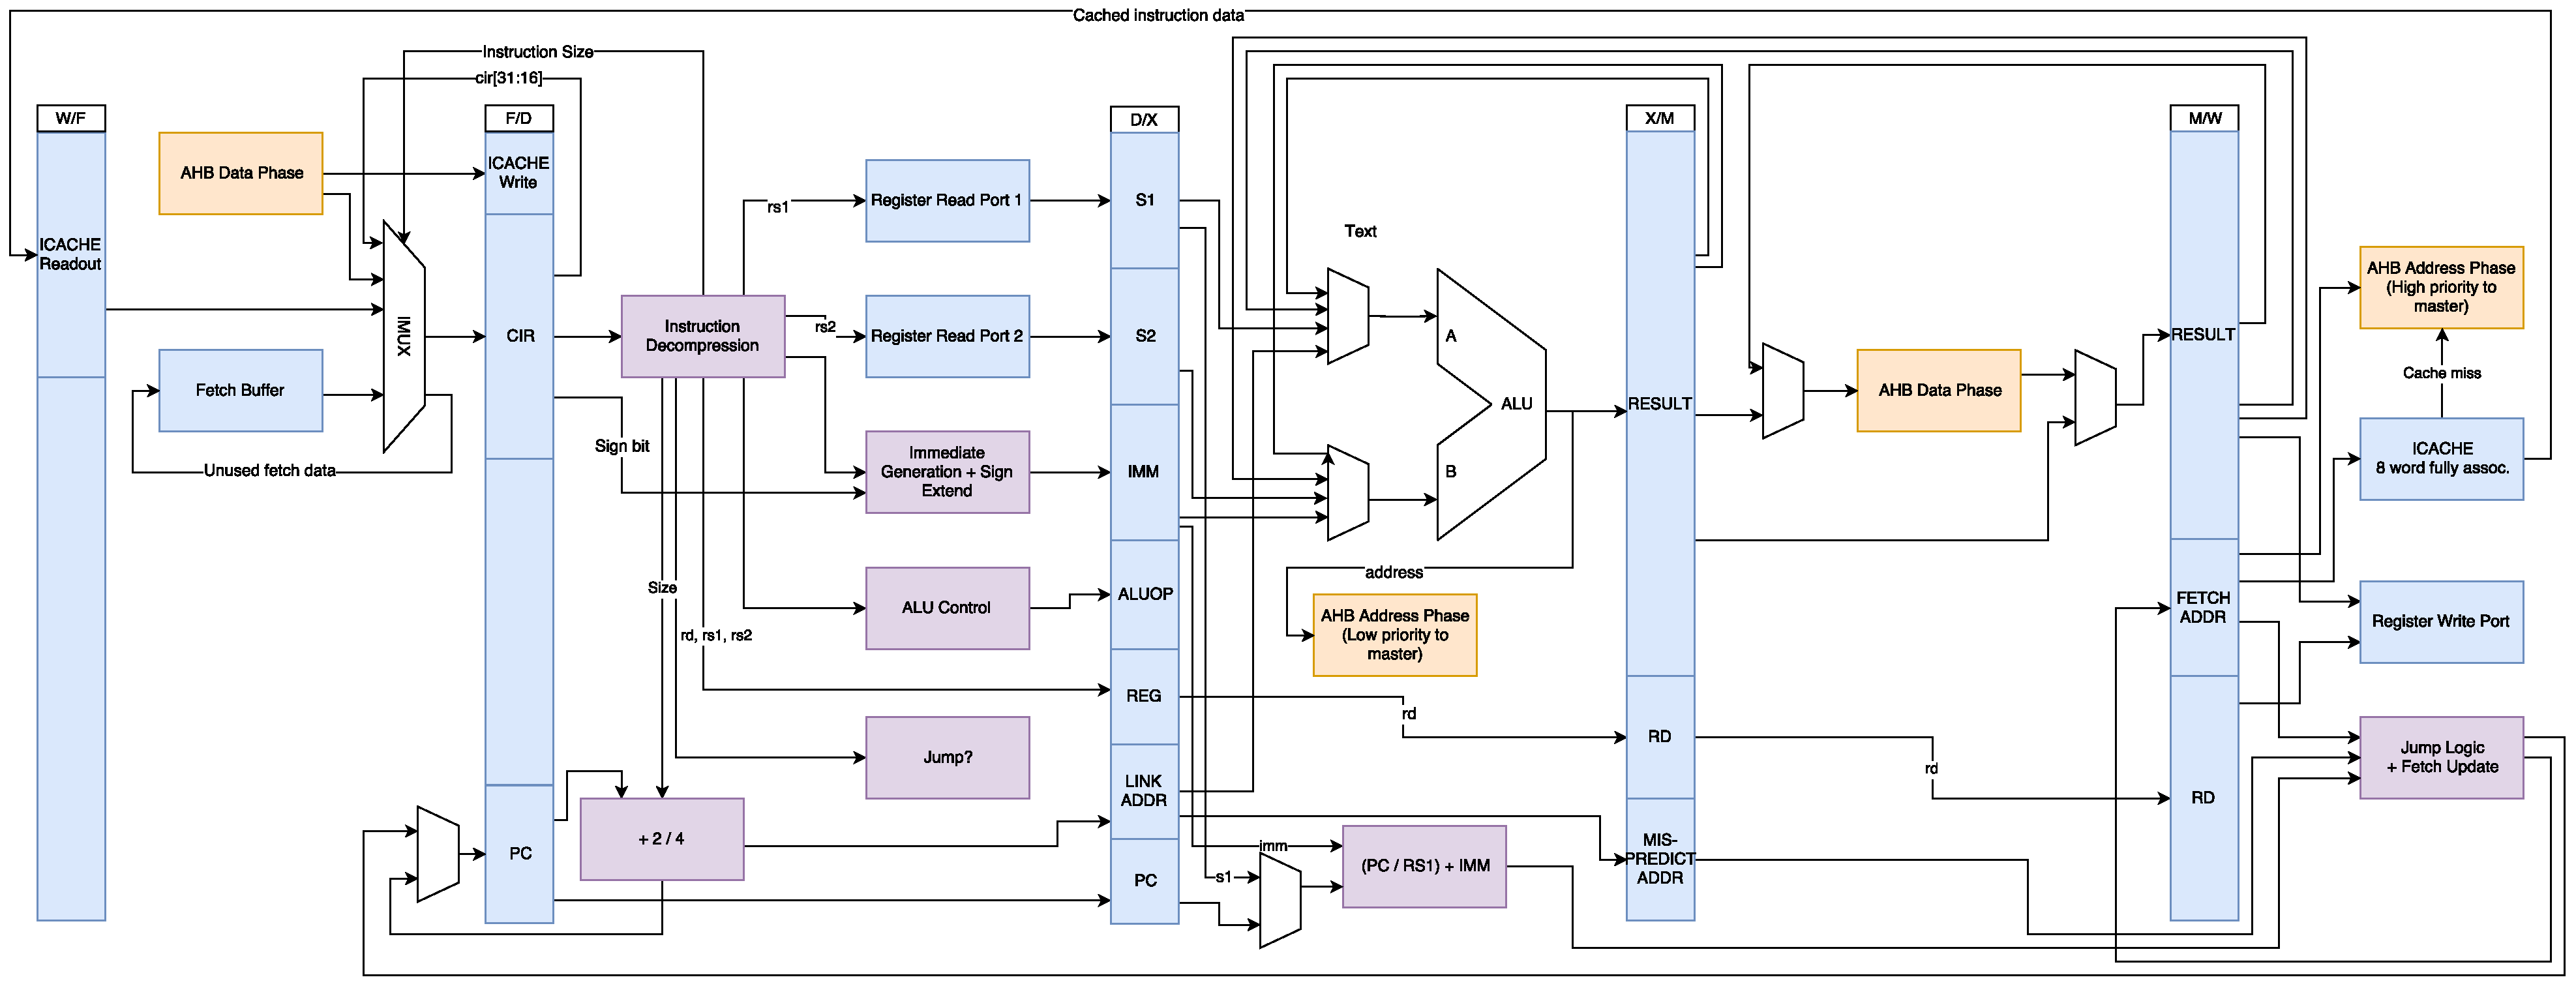
\includegraphics[width=\textheight]{diagrams/cpu_full.pdf}
			\captionof{figure}{ReVive architectural block diagram}
			\label{diagram:cpu_pipeline}
		\end{minipage}
	\end{sideways}
\end{center}

\newpage

\subsection{Fetch Logic}

\texttt{F} always provides \texttt{D} with 32 bits of fresh instruction data, in the canonical RISC-V order (halfword-wise little-endian). There are four sources:

\begin{itemize}
\item AHB busmaster with access to system memory map
\item \texttt{ICACHE}. A small, fully-associative cache with random eviction
\item An \texttt{F}-local buffer containing up to 32 bits of fetched, unused instruction data
\item The second halfword of the current instruction register of \texttt{D}, in the case that \texttt{D} found the last instruction to be 16-bit
\end{itemize}

The pipeline register \texttt{F} writes to, containing the 32 fresh instruction bits, is referred to internally as current instruction register or \texttt{CIR}.

AHB instructions fetches are \textit{always} word-sized, word-aligned. Internal buffering and muxes take care of building unaligned instruction bundles from this aligned data stream.

\subsubsection{Purpose of Fetch Buffer}

Between them, \texttt{ICACHE} and AHB provide \texttt{F} with 32 bits of fresh fetch data on every cycle (assuming that, on cache miss and \texttt{HREADY} low, \texttt{F} simply stalls), or with 0 bits if a fetch was not requested. \texttt{D} will consume either 32 or 16 bits of instruction data per cycle, and quickly determines this size by looking at the two LSBs of \texttt{CIR}; \texttt{F} can see the size of the instruction currently in \texttt{D}. 

Due to the pipelined nature of AHB, the decision of whether to fetch is made one cycle ahead of \texttt{F} itself, which ends up being in \texttt{W}. We aren't magicians: we use buffering to hide this latency cycle. On no-fetch cycles in \texttt{F} (having decided one cycle prior not to fetch), we will still need 32 bits of fetch data on hand to guarantee that we can refill \texttt{CIR} at the end of the cycle, once \texttt{D} has consumed up to 32 bits of instruction.

To summarise our state transitions:

\begin{itemize}
\item Fetch:
	\begin{itemize}
	\item 32-bit instruction in \texttt{CIR}: buffer level stays same
	\item 16-bit instruction in \texttt{CIR}: buffer level increases by 16
	\end{itemize}
\item No fetch:
	\begin{itemize}
	\item 32-bit instruction in \texttt{CIR}: buffer level decreases by 32
	\item 16-bit instruction in \texttt{CIR}: buffer level decreases by 16
	\end{itemize}
\end{itemize}

This suggests a simple rule: fetch if the buffer is not currently full. If we follow this rule, we guarantee that the buffer will have 0, 16 or 32 bits of data at all times.

TODO: consider performing 16-bit fetches if there is 16 bits of space in the buffer. The bus to main memory is only 16 bits wide, so executing 16 bit instructions with 32 bit fetches will only execute 2 cycles in every 3, due to the AHB wait state stalling \texttt{F}. Need to consider how this would interact with the cache.

\subsubsection{Sequential Code}

In sequential code, the \texttt{ICACHE} will be queried every cycle (unless the fetch buffer is full), during \texttt{W}, as to whether it has the next aligned word. We are able to guarantee that all AHB and \texttt{ICACHE} accesses are word aligned due to the operation of the fetch buffer in \texttt{F}.

The query response is combinatorial, and is used to decide whether to assert an AHB access during the address phase. Successful queries will result in cached read data appearing on the next clock edge, for use by \texttt{F}.

\texttt{F} is concurrent with the AHB data phase, except for a small muxing layer at the end which assembles the instruction word from AHB data, buffered data and cached data.

Following an unsuccessful \texttt{ICACHE} query, \texttt{F} will write the AHB data into the cache, evicting one word of its present contents. \textit{The same address must not appear more than once in the cache}, as the query logic is based on a non-priority sum of product encoder.


\subsubsection{Jumps}
\label{section:jumps}

When jumping or taking a branch, \texttt{F} invalidates its fetch buffer, and ignores present \texttt{CIR} contents. Aligned jumps are otherwise no different from sequential code: \texttt{ICACHE} is queried with the jump address, and AHB supplies the data if \texttt{ICACHE} does not have it.

Unaligned jumps (i.e., halfword-aligned but not word-aligned) are more painful, as we may need to perform two accesses to fetch the required data:

\begin{enumerate}
	\item \texttt{W} queries the cache with the address of the word containing the first instruction halfword
	\begin{itemize}
		\item If we hit \texttt{ICACHE}, we issue an AHB read to fetch the \textit{second} word in parallel with reading out from the cache
		\item If we miss, we issue an AHB read to fetch the first word from system memory.
	\end{itemize}
	\item On the next cycle, we have either 32 or 64 bits of fetch data available to \texttt{F}, depending on cache hit/miss
	\begin{itemize}
		\item The first halfword is useless
		\item If we have only 32 bits, then we put the second halfword into \texttt{CIR}, and assert a flag to inform \texttt{D} that only this halfword is valid
		\item If we have 64 bits, we forward the middle two halfwords to \texttt{CIR}, and stash the final halfword in the fetch buffer. Normal execution resumes.
	\end{itemize}
	\item If \texttt{CIR} was half-valid:
		\begin{itemize}
			\item \texttt{D} reports instruction was 16-bit: we got away with it.
			\item \texttt{D} reports 32-bit instruction: \texttt{D} stalls, \texttt{F} sends a full \texttt{CIR} based on new fetch data from this cycle.
		\end{itemize}
\end{enumerate}

\subsubsection{ICACHE Writeback}

The encoder logic used in the cache lookup does not give correct output if a tag appears multiple times in the cache (however, it is smaller/faster as a result). There is a behaviour pattern that could put \texttt{ICACHE} into an invalid state if we fetched from the same address on consecutive cycles:

\begin{enumerate}
	\item Miss on first cycle; \texttt{W} performs an AHB address phase.
	\item Writeback data not visible until end of this cycle; \texttt{W} performs duplicate AHB address phase.
	\item One copy of data has been written to \texttt{ICACHE}; another write is in progress. \texttt{W} hits \texttt{ICACHE} on this cycle, so no AHB address phase.
	\item The second write has put \texttt{ICACHE} into an invalid state; fetch behaviour is undefined from this point.
\end{enumerate}

Extreme care is required to avoid this pitfall. This sequence does not occur during normal execution: sequential code fetches are to incrementing addresses, and jumps (including jump-to-self) have a penalty cycle, which prevents the double-write behaviour. However, stalls must be treated carefully.

\subsubsection{Program Counter}

ReVive does \textit{not} use the program counter (\texttt{PC}) for code fetching, during sequential execution. It is used exclusively for the first fetch cycle of jumps/branches, the link value in \texttt{JAL(R)}, and branch mispredict recovery.

Instruction fetch takes place from a consecutive series of word-aligned addresses, as described in section \ref{section:jumps}. \texttt{F} feeds data back to the fetch control in \texttt{W} to indicate whether a new fetch is needed. \texttt{W} therefore never requires the value of \texttt{PC} during normal operation. However, during non-sequential execution, it does require a \texttt{PC} value. Bits [31:2] are used to set the new fetch address, and bit 1 is used to determine whether the first instruction is aligned or unaligned with the fetch. The difference is outlined in section \ref{section:jumps}: essentially, on an unaligned jump, the first 16 bits of the fetch data are ignored, and the hardware scrabbles to put together a valid instruction.

The true \texttt{PC} lives in \texttt{F}. It watches the size of instructions in \texttt{D}, and uses this to increment by 2 or 4 each cycle. \texttt{D} looks at this \texttt{PC} value when using its jump logic: it can either look at the value currently in the \texttt{PC} register, or the value due to be written to it at the end of the current clock. This gives the address of the instruction currently in \texttt{D}, and the address of the immediately following instruction, respectively. The first is used in the calculation of jump targets; the second is the link value used in \texttt{JAL(R)} and mispredict recovery.

\subsection{Jumps and Branches}


Due to the pipelined nature of AHB, we are unable to jump or to take branches in fewer than 2 cycles:

\begin{itemize}
\item Cycle 0: AHB address phase to fetch jump/branch instruction
\item Cycle 1: AHB data phase for fetch of jump/branch. Next instruction is in address phase concurrently.
\item Cycle 2: Jump/branch instruction is now available to \texttt{D}
	\begin{itemize}
		\item (Quickly) use to control the new address phase
		\item The immediately following instruction is already in data phase
	\end{itemize}
\item Cycle 3: data phase for jump target instruction
\end{itemize}


We've paid one penalty cycle in the pipeline (cycle 2), and also made one wasted code fetch.

Jumps are physically taken in \texttt{W}, directly in front of the fetch address generator. There are two reasons to jump:

\begin{itemize}
	\item Inspecting the \texttt{CIR} in \texttt{F/D} pipe register (\texttt{JAL}, speculated taken branches)
	\item Inspecting \texttt{X/M} pipe register (\texttt{JALR}, branch mispredict)
\end{itemize}

\texttt{JALR} (indirect jump) is taken later because it uses the register file and the ALU to compute its target.

If both of these sources attempt to jump in the same cycle, \texttt{X/M} takes priority, since it is executing an older instruction. In both cases, the part of the pipeline in the hazard shadow is invalidated; i.e., \texttt{W} $\to$ \texttt{F}, or \texttt{W} $\to$ \texttt{X}. Invalidation is performed by clobbering the pipeline control signals in such a way that these instructions will have no side effects.

This gives the following cycle costs, assuming full speculation:

\begin{center}
\begin{tabular}{l c}
\hline
Jump Type & Cycles (Execution + Penalty) \\
\hline
Direct jump & 2 \\
Predicted, non-taken branch & 1 \\
Predicted, taken branch (same as jump) & 2 \\
Indirect jump & 4 \\
Branch mispredict & 4 \\
\hline
\end{tabular}
\end{center}

The branch prediction scheme is static: take backward branches, and do not take forward branches.

\subsection{Operand Bypass}

ReVive provides a multiplexed operand bypass (forwarding) network. Register writes by a given instruction must always be visible to later instructions, even \textit{before} the first instruction reaches the register writeback stage. This is shown as multiplexers on the ALU inputs in figure \ref{diagram:cpu_pipeline}.

This removes, or at least shortens, read-after-write data hazards in the pipeline, and allows us to approach one clock-per-instruction execution rates. Without bypassing, only one instruction could be present in $\left\{ \texttt{D}, \texttt{X}, \texttt{M}, \texttt{W} \right\}$ at a time, giving a CPI of 4.

The following bypasses are available: (notation: pipe register $\to$ pipestage logic)

\begin{itemize}
	\item \texttt{X/M} $\to$ \texttt{X}
	\item \texttt{M/W} $\to$ \texttt{X}
	\item \texttt{M/W} $\to$ \texttt{M}
	\item \texttt{M/W} $\to$ \texttt{D} (internal bypass in register file for write port $\to$ read port)
\end{itemize}

To control the bypassing, some of the register specifiers from \texttt{CIR} are passed down the pipeline alongside the data. \texttt{rs1, rs2, rd} (operand sources and destination) are passed down as far as \texttt{X}. \texttt{rs2, rd} make it to \texttt{M}, and \texttt{rd} makes it to \texttt{W}.

These serve the following purposes:

\begin{itemize}
	\item \texttt{rd} is needed in \texttt{W} anyway, for performing the actual writeback
	\item \texttt{X} looks at the two operand source registers it depends on, and then glances across at the \texttt{rd}s awaiting writes in \texttt{M} (i.e. its own output) and \texttt{W} (i.e. a load output, or an \texttt{X} output one cycle prior).
	\item \texttt{M} Looks at the \texttt{src} register for a store (encoded in the \texttt{rd2} specifier field), and will look at the pending register write in \texttt{W}, which will be either a load result or a prior \texttt{X} result.
\end{itemize}

Architecturally, it may be preferable to perform these bypasses earlier, since RISC-V makes operand decode very simple, with fixed bitfield position for rd1, rd2. That is, put the muxes between the register file and the \texttt{D/X} pipe register, and move the taps to make the hazards work. However, we want the register file to support BRAM inference on iCE40 FPGAs, as we otherwise use about 15\% of the flops on the device just to implement the registers. iCE40s have a synchronous BRAM read port, so the muxes end up after the "pipe register", i.e. the BRAM output registers.

The upshot is:

\begin{itemize}
	\item Back-to-back ALU operations execute at 1 CPI
	\item Loads execute at 2 CPI if they are immediately required by the ALU. 1 CPI otherwise.
	\item Stores execute at 1 CPI
	\item In a load-store pair, the load takes only one cycle, since the \texttt{M} stage has cyclic forwarding
\end{itemize}

\subsection{Pipeline Stalling and Flushing}

Our terminology: stalling means a pipeline stage, along with prior stages, does not advance its state until some blocking condition has cleared. Flushing is when in-flight instructions in some stages are replaced with NOPs, and their results are discarded.

All stages stall on HREADY low, no matter which internal master instigated the current data phase. TODO: this is non-optimal. For example, if code fetch is stalled, stages \texttt{D,X,M} could still proceed. This would save one cycle in the case that \texttt{X} is stalled in a RAW hazard on \texttt{M}. We may save \textit{some} cycles on a jump/branch which would cause the current fetch data phase to be ignored; however, AHB does not allow us to assert a new address whilst the current address phase is in progress, so the whole pipe would still stall on the code fetch once the jump/branch is ready to be asserted. For now it seems best to proceed with the simple option.

Besides HREADY low, each stage may stall for the following reasons:

\begin{itemize}
	\item \texttt{F}: stall in \texttt{X}
	\item \texttt{D}: stall in \texttt{X}
	\item \texttt{X}:
	\begin{itemize}
		\item \texttt{W} needs the AHB busmaster
		\item RAW hazard on \texttt{M}
	\end{itemize}
	\item \texttt{M}: only on HREADY
	\item \texttt{W}:
	\begin{itemize}
		\item Writeback: only on HREADY
		\item PC generation: stalls when \texttt{X} stalls
	\end{itemize}
\end{itemize}

Pipeline bubbles are inserted into a pipe register by the rightmost stage in the stall chain. This stage creates the bubble by zeroing out the destination register field, memory op field, and any other fields which cause side effects. Under the above stall policy, only \texttt{X} will need to create bubbles: this ends up a single bubble, on an \texttt{M} $\to$ \texttt{X} RAW hazard.

\subsection{Unaligned Memory Accesses}

Alignment is the constraint that the address of a memory access be equal to zero, modulo some size. Where no size is specified, we refer to \textit{natural} alignment, i.e. modulo the size of this particular memory operation. RISC-V requires that memory is byte-addressable.

The RISC-V base ISA sizes instructions in 32-bit parcels, which must be 32-bit aligned; the compressed instruction extension relaxes this constraint to 16 and 16 bits. Data accesses range in size from single bytes to the machine word size, with no alignment requirements. 

ReVive uses AHB-lite for its bus interface. AHB-lite requires alignment of all accesses; this simplifies AHB-lite compatible hardware. The drawback for us is that, when programmers request a single unaligned access, the ReVive hardware must carry this out as multiple aligned accesses of smaller size. To avoid adding additional complexity to the CPU state machine, we handle this problem in two parts:

\begin{itemize}
	\item The CPU proceeds with an unaligned AHB transfer, blissfully unaware of the alignment requirements. This is already significantly complex.
	\item An additional busfabric component -- the \textit{aligner} -- sits between the CPU master port and the busfabric crossbar
	\begin{itemize}
		\item Single unaligned accesses by the aligner's master trigger multiple aligned accesses to its slave
		\item The aligner stalls its master using \texttt{HREADYOUT} during until the last bus cycle, whereupon it passes through the slave's \texttt{HREADYOUT}
		\item A shift register inside the aligner collates the results of multiple reads, or provides data for multiple writes
	\end{itemize}
\end{itemize}

We are able to simplify the CPU operation by reusing the existing AHB stall logic, although we may lose some speed by outsourcing the alignment logic. It's expected that this component will live inside a top-level CPU wrapper.

\begin{figure}[!htb]
\centering
\label{diagram:unaligned_accesses}
\caption{Aligner busfabric component}
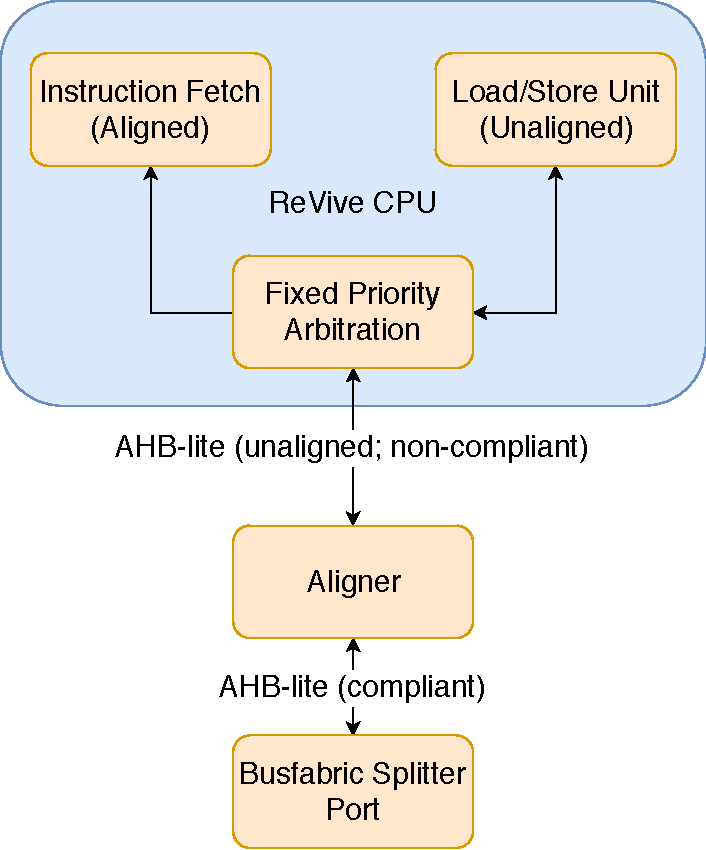
\includegraphics[width=0.4\textwidth]{diagrams/unaligned_accesses.pdf}
\end{figure}

\subsection{Pipeline Operation -- Worked Examples}

This section is included as much for my benefit as anything else. It describes the operation of all 5 pipeline stages for a few specimen instructions. I found it helpful to print out a few copies of figure \ref{diagram:cpu_pipeline} to trace out instructions with pen and paper.

\subsubsection{ADD}

Assembly: \texttt{add rd, rs1, rs2}

Pseudocode: \texttt{rd} $\leftarrow$ \texttt{rd1} $+$ \texttt{rd2}

\begin{enumerate}
	\item \texttt{F}
	\begin{itemize}
		\item Instruction can be either 16 or 32 bit
	\end{itemize}
	\item \texttt{D}
	\begin{itemize}
		\item Current values of source registers are read out from register file
		\item An internal bypass in the register file routes in the result of the instruction currently in \texttt{W}, if said instruction's \texttt{rd} matches our \texttt{rs1,rd2}, and the instruction generates a regfile write.
	\end{itemize}
	\item \texttt{X}
	\begin{itemize}
		\item Check the \texttt{rd} of \texttt{X/M} against our \texttt{rs1, rs2}. If there is a match:
		\begin{itemize}
			\item If \texttt{M} instruction is an ALU op: bypass it in
			\item If \texttt{M} instruction is a load: stall until it completes
		\end{itemize}
		\item Otherwise, check \texttt{rd} in \texttt{M/W}. If there is a match, bypass this result in.
	\end{itemize}
	\item \texttt{M}
	\begin{itemize}
		\item \texttt{add} is a no-op in \texttt{M}
		\item Our result is present in the pipe register, as well as our \texttt{rd}, and the fact that we are an ALU operation. Earlier pipe stages will forward our result as necessary
	\end{itemize}
	\item \texttt{W}
	\begin{itemize}
		\item Our result is pending write to the register file, and will be visible as of the next cycle
		\item \texttt{D} is able to bypass our result in due to internal regfile bypass. \texttt{X,M} can also bypass our result using the normal bypass network
	\end{itemize}
	\item Retirement
	\begin{itemize}
		\item The result has been written to the register file. The instruction has no further side effects.
	\end{itemize}
\end{enumerate} 


\subsubsection{JAL}

Pseudocode: \texttt{rd $\leftarrow$ PC + 2/4;  PC $\leftarrow$ PC $+$ imm}

(\texttt{JAL} has both 32-bit and 16-bit variants, so the value of the link address will vary.)


\begin{enumerate}
	\item \texttt{F}
	\begin{itemize}
		\item Whilst the jump is being fetched in \texttt{F}, the following instruction is entering the AHB address phase in \texttt{W}.
		\item This following fetch will be wasted, but we have no way of knowing this until we start to decode the jump instruction.
	\end{itemize}
	\item \texttt{D}
	\begin{itemize}
		\item This is a J-format instruction. It contains 20 bits of immediate data, which are sign-extended and effectively left-shifted by 1 by the immediate mux structure.
		\item \texttt{pc\_next} is passed on to \texttt{dx\_linkval}. ALU + muxes are configured to compute the sum of this value and \texttt{x0}.
		\item Immediate value is passed on as normal.
		\item \texttt{F} is stalled
	\end{itemize}
	\item \texttt{X}
	\begin{itemize}
		\item ALU passes link address to \texttt{X} result.
		\item Jump target adder computes \texttt{PC + imm}.
		\item Fetch update logic in \texttt{W} is flagged that \texttt{X} has a valid jump target. This is forwarded on to the fetch logic.
		\item \texttt{D} is stalled.
	\end{itemize}
	\item \texttt{M}
	\begin{itemize}
		\item New instruction is in \texttt{F}. Two penalty cycles were incurred by jump.
		\item The instruction is finished, but the link value continues on down the pipeline toward \texttt{W}. It is also available to the bypass network.
	\end{itemize}
	\item \texttt{W}
	\begin{itemize}
		\item Link address is written to register file.
		\item Target instruction is now in decode, and may use the link value via regfile bypass.
	\end{itemize}
\end{enumerate}


\subsubsection{JALR}

Pseudocode: \texttt{rd $\leftarrow$ PC + 2/4; PC $\leftarrow$ rs1 + imm}


\begin{enumerate}
	\item \texttt{F}
	\begin{itemize}
		\item Whilst the jump is being fetched in \texttt{F}, the following instruction is entering the AHB address phase in \texttt{W}.
		\item This following fetch will be wasted, but we have no way of knowing this until we start to decode the jump instruction.
	\end{itemize}
	\item \texttt{D}
	\begin{itemize}
		\item This is an I-format instruction. It contains 12 bits of immediate data, which are sign-extended but not shifted.
		\item \texttt{pc\_next} is passed on to \texttt{dx\_linkval}. ALU + muxes are configured to compute the sum of this value and \texttt{x0}.
		\item Immediate value is passed on as normal.
		\item \texttt{F} is stalled
	\end{itemize}
	\item \texttt{X}
	\begin{itemize}
		\item ALU passes link address to \texttt{X} result.
		\item Jump target adder computes \texttt{rs1 + imm}.
		\item Fetch update logic in \texttt{W} is flagged that \texttt{X} has a valid jump target. This is forwarded on to the fetch logic.
		\item \texttt{D} is stalled.
	\end{itemize}
	\item \texttt{M}
	\begin{itemize}
		\item New instruction is in \texttt{F}. Two penalty cycles were incurred by jump.
		\item The instruction is finished, but the link value continues on down the pipeline toward \texttt{W}. It is also available to the bypass network.
	\end{itemize}
	\item \texttt{W}
	\begin{itemize}
		\item Link address is written to register file.
		\item Target instruction is now in decode, and may use the link value via regfile bypass.
	\end{itemize}
\end{enumerate}

\subsubsection{LW and friends}

Pseudocode: \texttt{rd $\leftarrow$ mem[rs1 + imm]}

Two cases: aligned and unaligned. Aligned:


\begin{enumerate}
	\item \texttt{F}
	\begin{itemize}
		\item Nothing special to see here.
	\end{itemize}
	\item \texttt{D}
	\begin{itemize}
		\item This is an I-format instruction. It contains 12 bits of immediate data, which are sign-extended but not shifted.
	\end{itemize}
	\item \texttt{X}
	\begin{itemize}
		\item ALU computes \texttt{rs1 + imm}. This is the load address. AHB address phase starts immediately if master is not contested (timing should be okay...)
	\end{itemize}
	\item \texttt{M}
	\begin{itemize}
		\item AHB data phase takes place. Loaded word appears in \texttt{M/W} result register at end of cycle.
	\end{itemize}
	\item \texttt{W}
	\begin{itemize}
		\item Loaded data is written to register file.
	\end{itemize}
\end{enumerate}

Unaligned: Only \texttt{X} and \texttt{M} are different.

\begin{enumerate}
	\item \texttt{X}
	\begin{itemize}
		\item ALU computes \texttt{rs1 + imm}.
		\item First cycle: AHB address phase to \texttt{(rs1 + imm) \& \textasciitilde 0x3}. \texttt{F, D} stalled.
		\item Second cycle: AHB address phase to prev address + 4. \texttt{F, D} resume.
	\end{itemize}
	\item \texttt{M}
	\begin{itemize}
		\item Second cycle: store AHB data phase result in a word-sized local buffer.
		\item Third cycle: use muxes to build full load result from buffer, second data phase.
	\end{itemize}
\end{enumerate}

\texttt{SW} is even worse. Due to AHB alignment requirements, a word-store may have to be implemented as a byte store, halfword store and byte store.

\texttt{LH} will require either one halfword fetch, one word fetch, or two byte fetches depending on alignment.

\texttt{LB} can always be completed with a single fetch.



\subsection{Interrupts}

Interrupts and traps are implemented using the mispredict recovery hardware. They are precise and immediate; however, no state saving is carried out by the processor. The handler is responsible for saving any registers it uses on the stack, and restoring the state of the stack afterwards. The RISC-V ISA makes it possible for our handler to completely restore the processor state before exiting, but does not provide any mechanism to perform a return without first smashing the link register on handler entry.

The interrupt return mechanism is implemented with a small amount of ISA abuse: the hardware stashes the link address in an invisible architectural register during handler entry. The handler calls the magic instruction \texttt{JAL x0, 0} to jump back to this stashed \texttt{PC} value and therefore exit the interrupt. Hopefully not too much is lost by shadowing this instruction (jump to self without link).

This assumes that the programmer always maintains a valid stack pointer in \texttt{x2}, with enough space to save the registers. In practice this is not such an onerous task, and other processors such as Cortex-M0 make liberal use of stack operations on interrupt entry/exit.

\section{Graphics Pipeline}

\begin{figure}[!htb]
\centering
\caption{Block-level diagram of graphics pipeline}
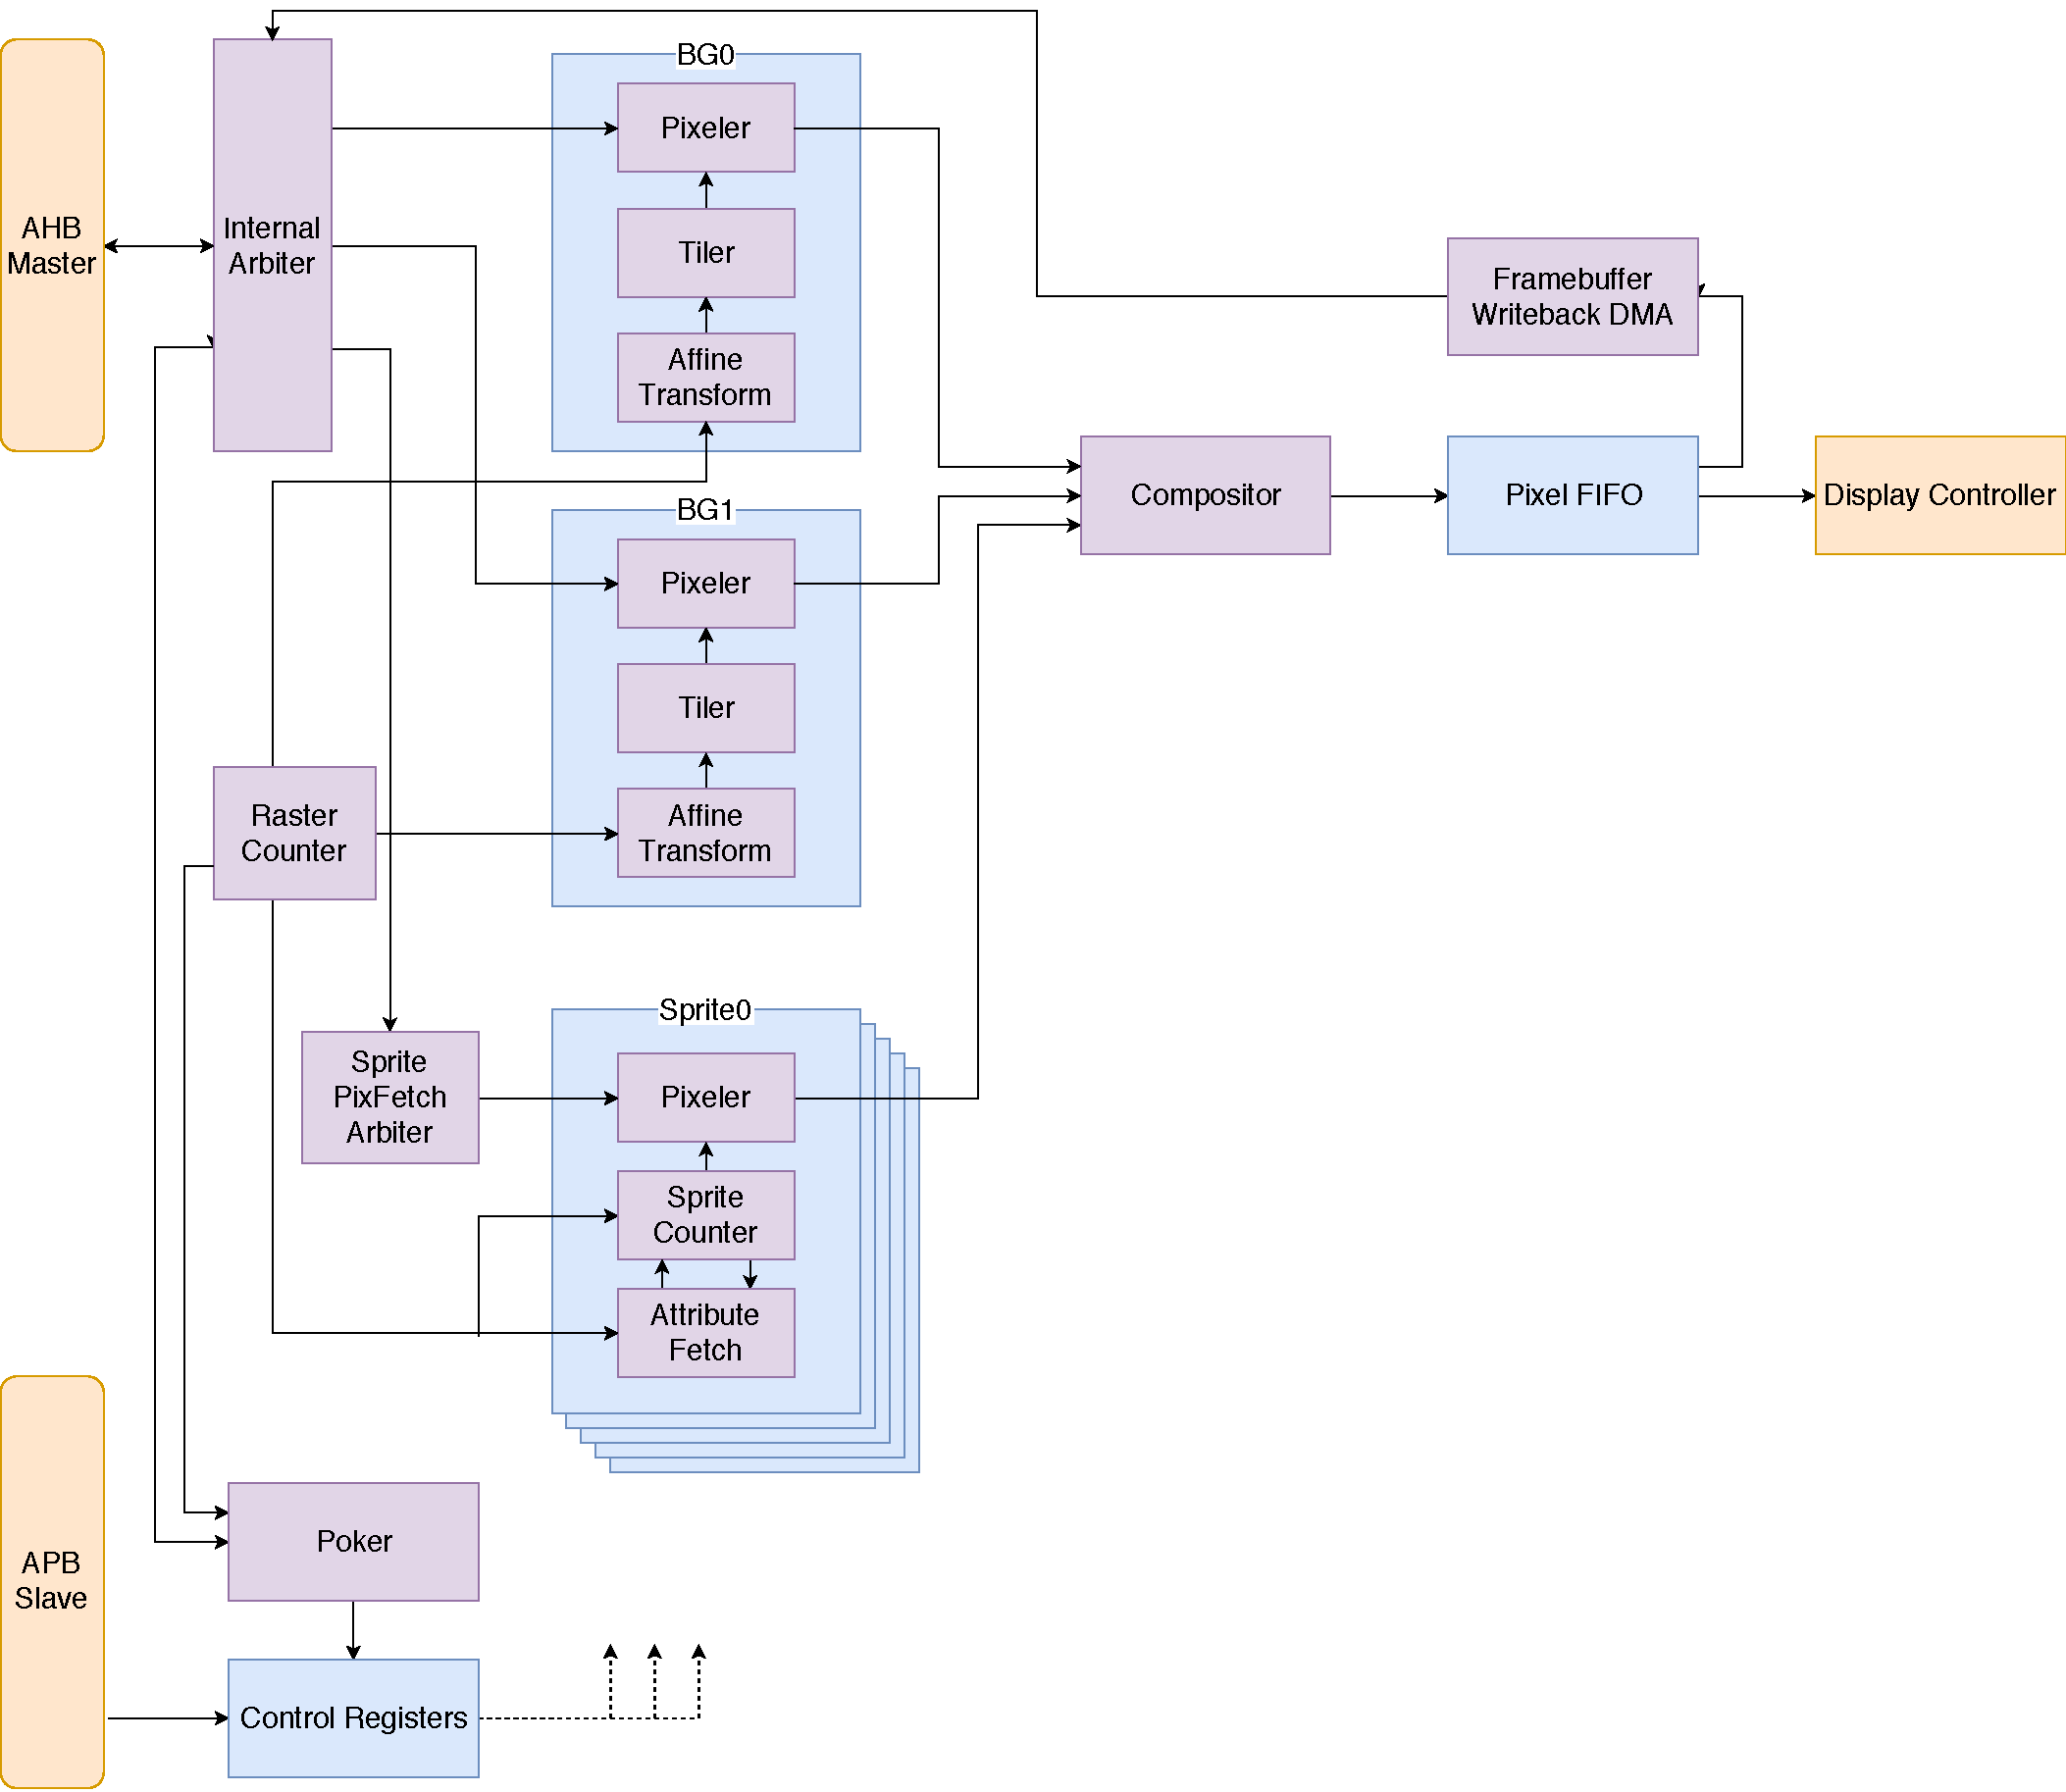
\includegraphics[width=0.9\textwidth]{diagrams/graphics.pdf}
\end{figure}

\section{Bus Fabric and Memory Subsystem}

\begin{figure}[!htb]
\centering
\label{diagram:crossbar_structure}
\caption{Module-level structure of AHBL crossbar}
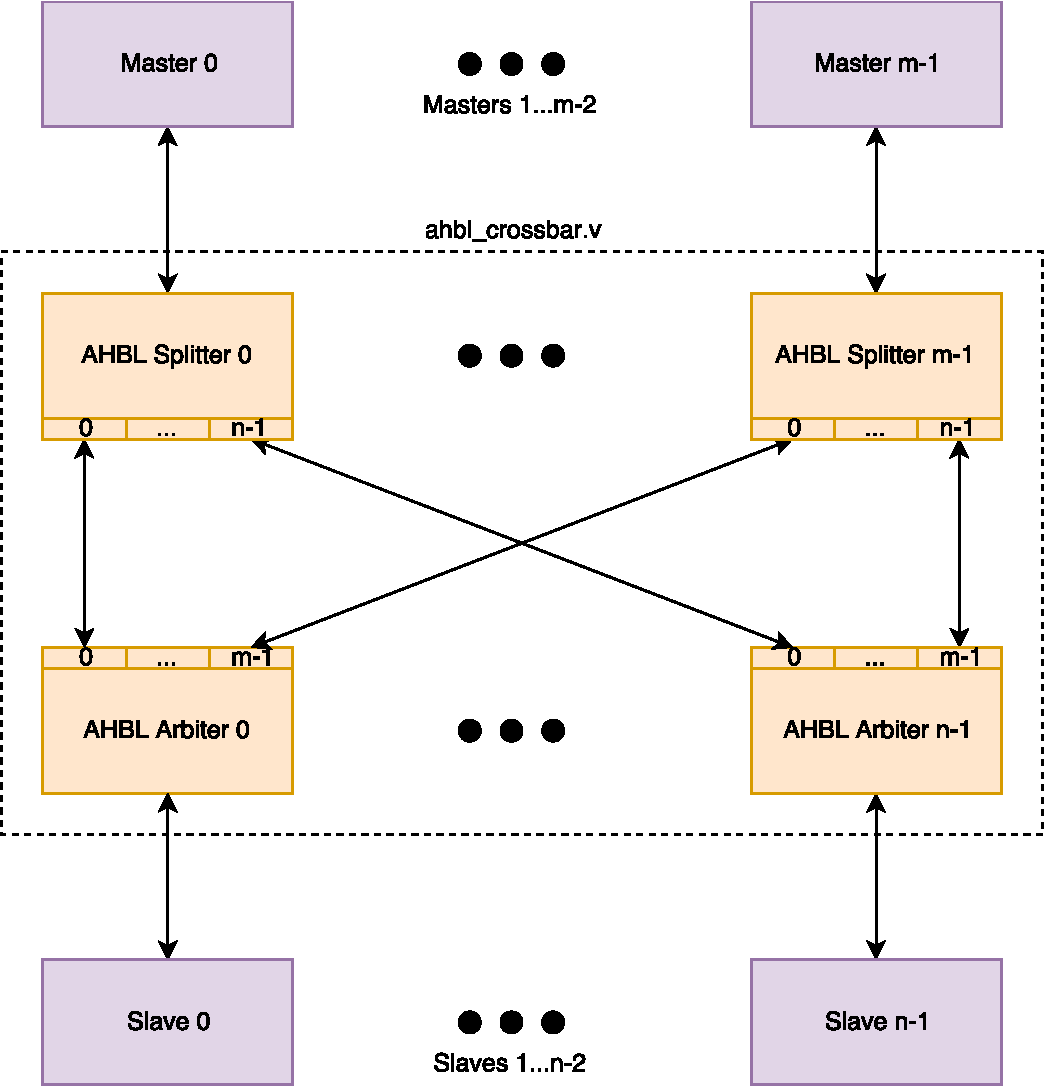
\includegraphics[width=0.6\textwidth]{diagrams/crossbar_structure.pdf}
\end{figure}

Figure \ref{diagram:crossbar_structure} shows the structure of the ahbl\_crossbar module (\texttt{hdl/busfabric/ahbl\_crossbar.v} in the code). To see how this fits into the overall system architecture, refer back to figure \ref{diagram:system_arch}, but in brief, it is used as a single-layer crossbar to connect the system masters, such as processor, to memories and peripherals. As shown, this module provides an independent AHB-lite datapath from each of $m$ masters to each of $n$ slaves. One master can address one slave at a time, and a slave can be in data-phase with one master at a time; subject to these constraints, up to $\min(m,n)$ independent data transfers can take place in a single machine clock cycle.

The modules are parameterised, but for FPGABoy they are instantiated with 32-bit address and data path widths.

\subsection{AHB-lite Brief Description}

It is recommended to read through ARM's AMBA 3 AHB-lite spec before looking over the code. This is included in the \texttt{reference} folder in the GitHub repository. However, if you are feeling brave, what follows is a brief outline of AHB-lite's signals and timing, which may provide sufficient background to understand the following sections.

AHB-lite is an asymmetric bus standard, where one or more masters assert transactions to one or more slaves. Each transaction can be either a read or a write. The size of a data cycle, encoded by \texttt{hsize}, is a power of two number of bytes, no larger than the width of the data bus. The standard requires all transactions to be naturally aligned, i.e. the modulo of address and transfer size is zero. This is in tension with the RISC-V ISA which allows transactions to have byte-alignment, so the load-store logic in the CPU may have to translate these into multiple AHB-lite transactions.

AHB-lite has separate data paths for read and write. This represents a move away from tristate logic in ASIC bus designs, and a lack of tristate logic in FPGAs.

AHB-lite transactions consist of two phases, named the address phase and the data phase. During the address phase, the master asserts signals which control the nature of the transfer, such as the address, whether the transfer is a read or write, protection/permission information, the width of the data, and so on. During the data phase, data is asserted on either the read or write data bus (\texttt{hrdata} and \texttt{hwdata}), but not both. The slave is able to insert wait states to extend the data phase, by deasserting the \texttt{hready\_resp} signal. \texttt{hready} indicates the final cycle of a data phase.

The central conceit of AHB-lite is that these two phases are pipelined, and therefore can take place simultaneously. Whilst the master is asserting or accepting data for bus cycle 0 (currently in data phase), it concurrently asserts address and control information for bus cycle 1 (currently in address phase). To avoid cluster-headaches, the two phases are kept totally concurrent, so deassertion of \texttt{hready\_resp} by a slave will also extend the master's \textit{address} phase.


\subsection{Bus Fabric Operation}

\texttt{hready} is a signal which tells masters and slaves that the current data phase is over. On a single-master busfabric, this is a global signal. It always propagates down from the master end of the busfabric, and is generated by performing some kind of filtering on \texttt{hready\_resp}s from the slaves.

\texttt{hready\_resp} (or \texttt{hreadyout} in some ARM docs) is a slave-driven signal indicating that this is the last cycle of the slave's current data phase.

On a single-master busfabric, the master will mux in the \texttt{hready\_resp} from the slave currently in the data phase, and pass this down as hready.  In our multi-master busfabric, a splitter functions as a single-master busfabric in its own right; the difference is that the splitter's master ports are connected to slave ports on arbiters, instead of slave ports on the actual slaves.  However, there is the additional requirement that, if a splitter is not currently data-phase active, it should mux \texttt{hready\_resp} based on \textit{address-phase} select. This is because, unlike on a single master system, there is no guarantee that the first address phase request in a series of bus cycles will receive a zero-wait state \texttt{hready\_resp}, as the slave may be engaged by another master. (Note this is not strictly in line with the standard, which requires a zero-wait-state \texttt{OKAY} response to a preceding \texttt{IDLE} address phase request).



\end{document}